\documentclass[11pt,a4paper]{article}
\usepackage[utf8]{inputenc}
\usepackage[T1]{fontenc}
\usepackage[spanish,es-tabla]{babel}
\usepackage[margin=2cm]{geometry}
\usepackage{array,longtable,graphicx}
\usepackage[hidelinks]{hyperref}
\newcolumntype{L}[1]{>{\raggedright\arraybackslash}p{#1}}
\setlength{\parskip}{3pt}
\setlength{\parindent}{0pt}
\setlength{\tabcolsep}{3pt}
\renewcommand{\arraystretch}{1.12}
\title{\vspace{-1.4cm}TA-IND-01\\\large IEEE 29148 y tipos de requisitos en Don Gerardo}
\author{Alan Andrés Aldas Zambrano\\\small Ingeniería de Requerimientos ISR-401, UTEQ, 4.º nivel, paralelo A}
\date{7 de noviembre de 2026}
\begin{document}
\maketitle
\vspace{-0.6cm}
\textbf{Borrador para revisión del estudiante.} Se organiza el relato aportado en el chat y se añaden propuestas identificadas como tales. El análisis normativo y parte de la formulación se prepararon con apoyo de IA. No se declara lectura personal de la norma, validación del dueño ni pruebas del software que no se hayan realizado.

\section{Resumen analítico aplicado al sistema}
Don Gerardo se desarrolló para un restaurante cuyo dueño, amigo del estudiante, necesitaba dejar de tomar pedidos a mano y reducir confusiones en cocina. El mesero elige platos, cantidades y mesa desde el teléfono o la tablet. La PC recibe la información y gestiona las comandas. Hay abonos por platos, rondas adicionales e inventario actualizado manualmente. El registro de ventas es básico, sin integración con facturación electrónica del SRI. Este contexto procede del estudiante; no se presenta como entrevista formal ni como una auditoría del negocio.

\subsection{Necesidad y requisito bien formado}
IEEE 29148 define requisito en 3.1.19 y aborda su construcción en 5.2.4 \cite{iso29148}. Para este caso, decir que la cocina necesita orden expresa el problema, pero no identifica por sí solo qué debe registrar la aplicación. El ejemplo del estudiante es más concreto: dos hamburguesas para una mesa, una con observación sin cebolla. Así se puede comparar lo solicitado con lo guardado e impreso. El restaurante no necesita solo una pantalla vistosa: necesita que cocina y el mesero reconozcan el mismo pedido.

Una afirmación como imprimir rápido tampoco fija cuándo empieza o termina la medición. El estudiante propuso tres segundos hasta el inicio de impresión, basándose en su experiencia. El borrador separa esa observación de una prueba con cronómetro. La condición de impresora libre es una propuesta para delimitar el escenario; todavía debe aceptarla el estudiante y el dueño. Si ya hay una comanda imprimiéndose, la espera pertenece a otro escenario y no se puede prometer el mismo tiempo sin comprobarlo.

\subsection{Calidad de cada enunciado}
El apartado 5.2.5 enumera nueve características: necesario, apropiado, no ambiguo, completo, singular, factible, verificable, correcto y conforme \cite{iso29148}. Su aplicación no consiste en marcar casillas porque el texto suene técnico. En Don Gerardo, la mesa y las cantidades son necesarias para entregar lo que se pidió. El nivel debe permitir definir la necesidad sin imponer detalles internos que el dueño no pidió. Para evitar ambigüedad, se diferencia una comanda original de una copia solicitada. La información debe ser suficiente para reconocer el pedido; decir que salga detallado deja abiertos los campos que se imprimirán.

La singularidad obliga a separar necesidades que cambian por razones diferentes. Registrar un pedido, cobrarlo y modificar inventario no son una sola función, aunque compartan datos. Un abono sí puede tratarse como una operación única con condiciones: selecciona platos pendientes y actualiza el saldo sin cobrarlos dos veces. La factibilidad del límite temporal depende de la impresora, red y carga; las capturas no demuestran ese desempeño. La verificabilidad mejora al comparar valores concretos. La corrección exige confirmar que el dueño necesita esos valores, y la conformidad permite usar identificadores, el verbo deberá y un formato constante.

\subsection{Calidad del conjunto y lenguaje}
El apartado 5.2.6 trata completitud, consistencia, factibilidad, comprensión y posibilidad de validación del conjunto; 5.2.7 advierte contra lenguaje ambiguo \cite{iso29148}. Aquí los abonos y las rondas deben ser compatibles: una ronda nueva incrementa el pendiente sin borrar los platos pagados. También hay que usar pedido, ronda y comanda con un significado estable. De otro modo, una reimpresión podría confundirse con una venta nueva. Revisar un requisito aislado no detectaría necesariamente esa contradicción.

El conjunto todavía tiene límites de validación. El estudiante afirma que el inventario se descuenta manualmente; por eso no se añade una receta automática por plato. También explicó una reconexión rápida, pero no se distinguió si falló internet, wifi o la impresora. Se propone evaluar la cola ya guardada en caja, sin asegurar que un teléfono desconectado del wifi puede transmitir. Los términos siempre, todo validado, cómodo y no se traba deben reemplazarse por condiciones y criterios observables. La propuesta de tres segundos, por ejemplo, tiene una unidad y un evento final definidos.

\subsection{Clasificación, evidencia y revisión}
El tipo es un atributo de organización en 5.2.8.2; los ejemplos de 5.2.8.3 distinguen funciones, interfaces, proceso, calidad y usabilidad, entre otros \cite{iso29148}. Este borrador utiliza esos cinco grupos. Una restricción no es automáticamente una función: la definición 3.1.7 permite reconocer límites impuestos. Que los dispositivos actuales compartan wifi es contexto observado; convertirlo en obligación futura requiere acuerdo. No se inventa una tecnología exigida por el dueño para completar una categoría.

Las propiedades de calidad se relacionan con ISO/IEC 25010:2023 \cite{iso25010}. Un criterio de integridad de precios no se demuestra solo porque el mesero no vea el botón: deben verificarse las rutas por las que podría intentar cambiarlos. Tampoco la palabra COPIA prueba que no exista duplicación automática. La revisión debe relacionar cada necesidad con un caso que pueda fallar. IREB distingue el trabajo de requisitos de la mera producción de documentos y presenta revisión y validación como actividades para detectar diferencias entre lo escrito y lo necesario \cite{ireb2024}. Por eso las tres capturas se usan como evidencia de interfaz, no como resultados de seguridad o rendimiento.

\section{Glosario aplicado}
Definiciones breves parafraseadas de la cláusula 3; los ejemplos son del caso \cite{iso29148}.
\begingroup\scriptsize\renewcommand{\arraystretch}{1.12}
\begin{longtable}{|L{3.2cm}|L{4.6cm}|L{7.4cm}|}
\hline\textbf{Término y apartado} & \textbf{Definición breve} & \textbf{Ejemplo propio del sistema} \\\hline
Requisito (3.1.19) & Necesidad expresada con condiciones. & Identificar la mesa en la comanda. \\ \hline
Condición (3.1.6) & Circunstancia en que se exige algo. & Impresora encendida, con papel y libre. \\ \hline
Restricción (3.1.7) & Límite impuesto a la solución o al trabajo. & Exigir una red local sería una restricción si se acuerda; hoy es contexto. \\ \hline
Escenario operativo (3.1.17) & Secuencia de interacción en un uso previsto. & Mesero selecciona, envía y cocina recibe. \\ \hline
Operador (3.1.18) & Quien realiza operaciones del sistema. & El cajero registra un abono. \\ \hline
Elicitación (3.1.20) & Identificación sistemática de necesidades. & Preguntar qué apartados necesita cocina. \\ \hline
Verificación de requisitos (3.1.26) & Revisión de su buena formulación. & Revisar que rápido tenga medida y límite. \\ \hline
Validación de requisitos (3.1.25) & Confirmación de que expresan la necesidad correcta. & Dueño revisa el ejemplo de comanda. \\ \hline
Interesado (3.1.28) & Persona u organización con interés en el sistema. & Dueño, mesero y personal de cocina. \\ \hline
Sistema de interés (3.1.32) & Sistema que se toma como objeto del análisis. & App de mesero, API, caja y cola de impresión en este alcance. \\ \hline
\end{longtable}
\endgroup

\section{Requisitos, clasificación y versiones corregidas}
F = funcional; I = interfaz; P = proceso; Q = calidad; U = usabilidad/calidad en uso como tipo de 5.2.8.3. Se cubren cinco tipos y seis requisitos con criterio de calidad (R09--R14). Los borradores iniciales son formulaciones de trabajo, no citas literales. La columna corregida es la versión vigente del borrador; no prueba implementación. Las pruebas indicadas son propuestas pendientes de ejecutar con datos ficticios en entorno aislado. R07, R08, R13 y las condiciones numéricas no confirmadas requieren aprobación del estudiante y del dueño. En R13 la prueba de desempeño de usuarios orienta la evaluación de interacción; no se afirma que ISO 25010 defina el modelo de calidad en uso.

\begingroup\footnotesize
\begin{longtable}{|L{1.1cm}|L{3.2cm}|L{6.2cm}|L{4.7cm}|}
\hline
\textbf{ID / tipo} & \textbf{Versión inicial y defecto} & \textbf{Versión corregida} & \textbf{Métrica o criterio de aceptación} \\\hline
\endfirsthead
\hline
\textbf{ID / tipo} & \textbf{Versión inicial y defecto} & \textbf{Versión corregida} & \textbf{Métrica o criterio de aceptación} \\\hline
\endhead
R01 / F & Los platos y la mesa. Faltan cantidad y responsable (C). & El sistema deberá permitir al mesero registrar un pedido con una mesa, platos, cantidades enteras positivas y observaciones opcionales por plato. \textit{Origen: Relato.} & Guardar 2 hamburguesas, una sin cebolla, para mesa 3; recuperar exactamente mesa, cantidad e indicación. \\ \hline
R02 / F & Que la comanda salga detallada. Detallada es subjetivo (U,V). & Al enviar un pedido o una ronda no vacíos a cocina, el sistema deberá generar su comanda solo con las líneas enviadas, mesa, cantidades y observaciones agrupadas por área de preparación. \textit{Origen: Relato.} & Comparar 3 pedidos de prueba con las comandas: coincidencia de datos y apartados de parrilla, moros o entradas cuando correspondan. \\ \hline
R03 / F & Solo lo nuevo, como nueva ronda. No se identifica qué se conserva (C). & Al añadir una ronda a una mesa con pedido abierto, el sistema deberá incorporar su importe al saldo pendiente conservando los abonos anteriores. \textit{Origen: Relato.} & Mesa con \$5 pendientes: añadir \$8 y comprobar saldo \$13 y abonos anteriores sin cambios. \\ \hline
R04 / F & Se paga el plato de diez y queda cinco. Falta identificar la operación (C). & El sistema deberá permitir al cajero registrar un abono por platos seleccionados y actualizar el saldo de la mesa descontando únicamente el importe de esos platos pendientes. \textit{Origen: Relato.} & Con platos de \$10 y \$5, pagar el de \$10; saldo \$5 y sin permitir cobrar otra vez ese plato. \\ \hline
R05 / F & Reimprimir cuando se pierde. No distingue original de copia (C). & Al solicitar una reimpresión de un pedido existente desde la app del mesero, el sistema deberá imprimir la misma comanda con la palabra COPIA en la parte superior. \textit{Origen: Relato.} & Reimprimir una comanda: conservar su identificador y detalle, mostrar COPIA y no aumentar el saldo de la mesa. \\ \hline
R06 / F & Que no ofrezca un plato que se acabó. Falta responsable y alcance (C). & El sistema deberá permitir al usuario autorizado de escritorio marcar un plato como no disponible e impedir que se agregue a nuevos pedidos después de actualizar el menú del mesero. \textit{Origen: Relato con alcance propuesto.} & Deshabilitar un plato de prueba, actualizar el menú y verificar que no puede añadirse; no se modifican pedidos ya enviados. \\ \hline
R07 / I & Todo funciona por una API. Describe tecnología sin datos de intercambio (C,V). & La interfaz entre móvil y caja deberá transportar el identificador de pedido y ronda, mesa, líneas de plato, cantidades y observaciones, y devolver confirmación asociada al mismo identificador. \textit{Origen: Propuesta de contrato.} & Inspeccionar un mensaje de prueba y su confirmación: todos los campos presentes, misma mesa e identificador en ambos extremos. \\ \hline
R08 / P & Actualizar conforme pide el dueño. No fija cuándo se valida (C,V). & Antes de publicar un cambio del formato de comanda, el responsable del desarrollo deberá registrar la revisión del dueño sobre un ejemplo sin datos de clientes y conservar su aceptación o sus correcciones. \textit{Origen: Propuesta de proceso.} & Para un cambio, inspeccionar ejemplo, fecha y respuesta real del dueño antes de liberar la versión; no fabricar aceptación. \\ \hline
R09 / Q & De dos a tres segundos. No distingue inicio, final ni cola (U,C). & Con red local estable e impresora térmica libre, encendida y con papel, la impresión deberá comenzar como máximo 3 segundos después de Enviar a cocina para pedidos de hasta 30 líneas de productos. \textit{Origen: Límite del estudiante; condiciones propuestas.} & 30 envíos separados, alternando teléfono y tablet: 30/30 inicios en tiempo menor o igual a 3 s. Medir desde pulsación hasta movimiento de papel. ISO: eficiencia de desempeño, comportamiento temporal. \\ \hline
R10 / Q & Que no imprima dos veces. No distingue reintento y copia solicitada (U). & El sistema deberá mantener una sola comanda original por identificador de pedido y ronda ante reintentos del mismo envío, sin impedir reimpresiones marcadas como COPIA. \textit{Origen: Necesidad relatada; prueba propuesta.} & 30 pedidos, repetir 3 veces cada envío: 30 originales y cero duplicados accidentales. Excluir las copias solicitadas. ISO: fiabilidad, tolerancia a fallos. \\ \hline
R11 / Q & Conserva el pedido y al reconectar imprime. No delimita qué conexión ni alcance (U,C). & El sistema deberá recuperar el 100 por ciento de los pedidos ya guardados en la cola de impresión de caja tras una interrupción de comunicación con la impresora, sin alterar sus datos. \textit{Origen: Propuesta; no acredita operación móvil sin wifi.} & En entorno aislado, dejar 10 comandas en cola, cortar y restablecer la comunicación: recuperar 10/10, datos iguales y ningún original extra. Sin plazo de recuperación afirmado. ISO: fiabilidad, recuperabilidad. \\ \hline
R12 / Q & Los meseros no entran a caja. Ocultar pantalla no acredita permisos (V). & El sistema deberá rechazar el 100 por ciento de los intentos de modificar precios o registrar cobros realizados con cuentas de mesero, conservando precios y saldos sin cambios. \textit{Origen: Permisos relatados; prueba propuesta.} & 20 intentos de cada operación con mesero, tanto por interfaz como por API si la operación se expone: 40/40 rechazados. ISO: seguridad, integridad. \\ \hline
R13 / U & Que sea cómodo para el mesero. Cómodo es subjetivo (U,V). & En una prueba de primer uso, al menos 4 de 5 participantes con tareas de mesero deberán registrar y enviar un pedido de tres platos para una mesa, con una observación, sin ayuda externa en un máximo de 2 minutos. \textit{Origen: Propuesta de evaluación; participantes no reclutados.} & Éxitos correctos sin ayuda y en tiempo / 5, mínimo 80 por ciento; medir desde menú inicial con sesión hasta confirmación. Registrar fallos y abandonos. ISO orientativa: capacidad de interacción, aprendizaje. \\ \hline
R14 / Q & Que los pedidos no se mezclen. No define comparación ni muestra (C,V). & El intercambio entre móvil y caja deberá conservar el 100 por ciento de los identificadores, mesas, platos, cantidades y observaciones de cada pedido confirmado, incluidos envíos cercanos de los dos dispositivos. \textit{Origen: Necesidad relatada; prueba propuesta.} & 30 pares de pedidos de mesas distintas desde teléfono y tablet; 60/60 registros iguales a origen y cero líneas asignadas a otra mesa. ISO: compatibilidad, interoperabilidad. \\ \hline
R15 / F & Que todo esté validado en inventario. Todo no identifica la regla (U,V). & Al registrar una salida manual de un insumo, el sistema deberá aceptar solo una cantidad positiva no mayor a la existencia disponible y conservar la existencia anterior cuando rechace la operación. \textit{Origen: Confirmación verbal; no prueba ejecutada.} & Con 5 litros, intentar salida de 8 y de -1: rechazar y conservar 5; registrar salida de 2: existencia 3. \\ \hline
\end{longtable}
\endgroup

\clearpage
\section{Autoevaluación de las nueve características}
La revisión textual utiliza 5.2.5 y 5.2.7 \cite{iso29148}. En cada fila anterior se conserva la formulación inicial, se identifica el defecto y se escribe la corrección. C = completo; U = no ambiguo; V = verificable. No se realizaron las pruebas de aceptación.

La siguiente matriz aplica los nueve criterios a cada versión corregida: N = necesario; A = apropiado; U = no ambiguo; C = completo; S = singular; F = factible; V = verificable; Co = correcto; T = conforme al formato. R indica revisión de redacción sin defecto adicional detectado; P indica pendiente de confirmar con evidencia o con el dueño. R no significa prueba aprobada ni certificación de cumplimiento. R01--R06 y R15 derivan del relato del estudiante; las propuestas nuevas no se dan por necesidades aceptadas.
\begingroup\scriptsize
\begin{longtable}{|c|c|c|c|c|c|c|c|c|c|}
\hline ID & N & A & U & C & S & F & V & Co & T \\\hline
R01 & R & R & R & R & R & P & R & P & R \\ \hline
R02 & R & R & R & R & R & P & R & P & R \\ \hline
R03 & R & R & R & R & R & P & R & P & R \\ \hline
R04 & R & R & R & R & R & P & R & P & R \\ \hline
R05 & R & R & R & R & R & P & R & P & R \\ \hline
R06 & R & R & R & R & R & P & R & P & R \\ \hline
R07 & P & R & R & R & R & P & R & P & R \\ \hline
R08 & P & R & R & R & R & P & R & P & R \\ \hline
R09 & R & R & R & R & R & P & R & P & R \\ \hline
R10 & R & R & R & R & R & P & R & P & R \\ \hline
R11 & P & R & R & R & R & P & R & P & R \\ \hline
R12 & R & R & R & R & R & P & R & P & R \\ \hline
R13 & P & R & R & R & R & P & R & P & R \\ \hline
R14 & P & R & R & R & R & P & R & P & R \\ \hline
R15 & R & R & R & R & R & P & R & P & R \\ \hline
\end{longtable}
\endgroup
Los P de factibilidad requieren comprobar la plataforma, red, impresora y procedimientos de prueba; los de corrección requieren aceptación del responsable del restaurante. Las ambigüedades detectadas se resolvieron en el texto propuesto, pero las decisiones nuevas no se presentan como acordadas. Por ejemplo, no se equipara ocultar un botón con bloquear una operación y no se aplica el límite de impresión a una cola ocupada sin medirla.

\section{Reflexión basada en el relato del estudiante}
La parte que más costó fue definir las comandas. Al principio se quería dejar de tomar pedidos a mano y evitar confusiones, pero durante el uso aparecieron detalles nuevos: un apartado para parrilla, otro para moros y otro para entradas. Esos apartados eran importantes porque la cocina trabaja por áreas y cada una necesita identificar lo que debe preparar. La impresión no debía limitarse a enumerar platos; también tenía que conservar mesa, cantidades e indicaciones.

El estudiante explicó que esos ajustes se hicieron sobre la marcha y exigieron nuevas actualizaciones. No se afirma que hubiera un prototipo aprobado antes de programar ni se inventa cuánto tiempo se perdió. Su aprendizaje es preguntar desde el inicio, con más detalle, qué debe aparecer en la comanda y cómo se organiza el trabajo de cocina. Conocer esos datos antes ayudaría a concretar mejor el requisito y a distinguir un cambio necesario de un detalle que simplemente no se preguntó.

La revisión también mostró que expresiones como rápido o todo validado no bastan para una especificación. El estudiante observó respuesta ágil, pero reconoció que no había medido la espera en cola. La propuesta de tres segundos debe separarse de una garantía comprobada. Este informe conserva sus observaciones y marca las pruebas y decisiones que todavía necesitan confirmación. Esta reflexión organiza sus respuestas con apoyo de redacción; requiere su lectura final antes de presentarse como conclusión personal.

\section{Evidencias de interfaz}
Se tomaron tres capturas reales en una sesión asistida. Los formularios de pedido e inventario se abrieron y cerraron sin guardar. El acceso lo realizó el estudiante. No se crearon pedidos, cobros ni cambios de inventario. No se detectó la API escuchando en el puerto 5206; por tanto, las imágenes no prueban el flujo móvil, seguridad ni tiempos. Los originales que contienen nombres de proveedores no se publican. Los hashes y el alcance figuran en \texttt{EVIDENCIAS.md}.

\begin{figure}[htbp]
\centering
\begin{minipage}{0.38\textwidth}\centering
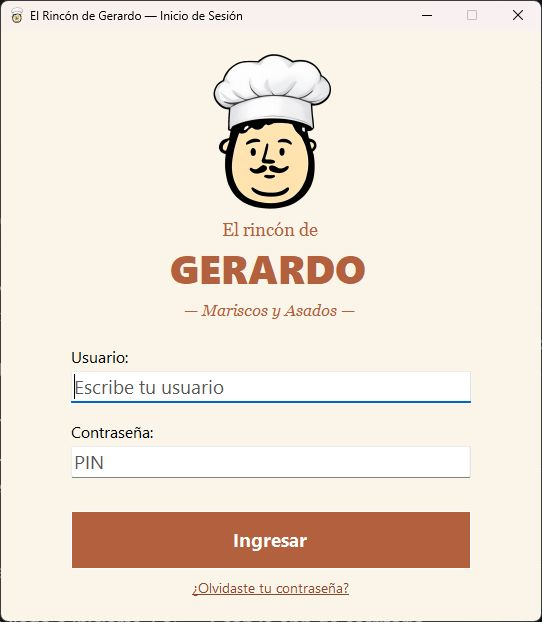
\includegraphics[height=4.4cm]{figuras/01_inicio_sesion.png}
\end{minipage}\hfill
\begin{minipage}{0.56\textwidth}\centering
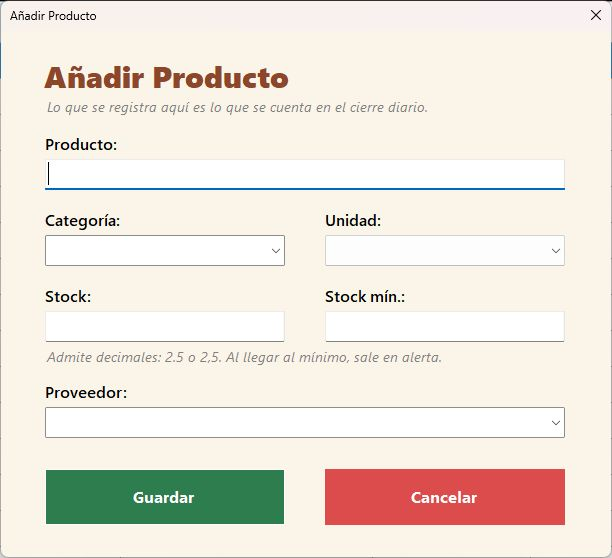
\includegraphics[height=4.4cm]{figuras/02_formulario_inventario.png}
\end{minipage}
\caption{Acceso y formulario de inventario sin credenciales ni datos de proveedores.}
\end{figure}
\begin{figure}[htbp]
\centering
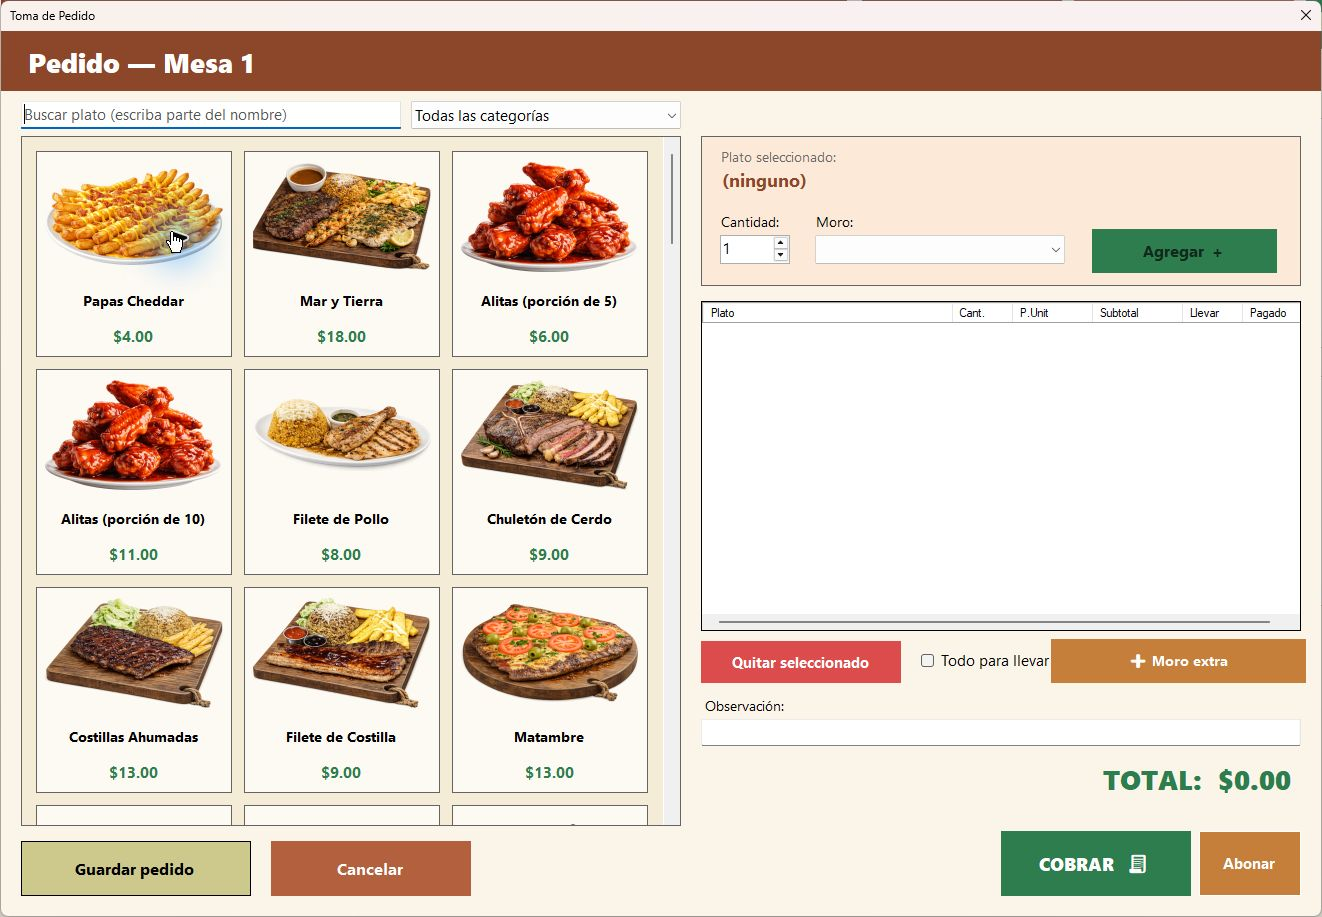
\includegraphics[width=0.88\textwidth]{figuras/03_toma_pedido.png}
\caption{Toma de pedido para una mesa libre, sin guardar operaciones.}
\end{figure}
\clearpage
\section{Uso de IA y estado del borrador}
Se utilizó ChatGPT/Codex para organizar el relato del estudiante, explicar conceptos, redactar este borrador y comprobar el documento. El estudiante aportó el contexto, las funciones descritas y la experiencia de cambios en comandas. La versión exacta del modelo no consta en el registro. Se contrastaron los apartados normativos y las referencias, se inspeccionaron capturas y se compiló el PDF. El borrador requiere revisión y redacción personal donde lo exige la guía; no declara una lectura de primera mano del estudiante todavía no acreditada ni limita la ayuda a ortografía. No se afirma que este alcance haya sido autorizado por el docente. El registro del sistema en el foro no está confirmado.

\bibliographystyle{IEEEtran}
\bibliography{referencias}
\end{document}
